\section{Projeto}

\subsection{Projeto de Processos}

O projeto de processo tem como objetivo criar soluções funcionais para atender as necessidades das pessoas por meio da organização dos recursos ou atividades que interfere no produto ou serviço que estão sendo prestados. Projeto de serviço e projeto de processo são interligados, porque os dois se interferem. Para ter um bom projeto de processo e terá alto desempenho na quantidade, pontualidade, rapidez e custo do serviço prestado ou do produto.

A fábrica Bom Sabor divulga o seu produto por meio de visitas pessoais ou por telefone ou são contatados.
Pro meio de ligações telefônicas ou visita, os pedidos são feitos, e anotados. A empresa recebe pedidos de forma não uniforme, a quantidade de pedidos varia, podendo assim variar junto a eficiência de entrega do produto, que é feita pela própria empresa, e o período de entrega é também de segunda a sexta. A produção do pastel é feita de acordo com os pedidos dos clientes, ou seja, só produzem o pastel depois de feito o pedido. A empresa tem onde armazenar os pasteis, na câmara fria, porem alguns pasteis não têm um longo prazo de validade por causa dos recheios. O recheio e a massa do pastel é produzido pela própria empresa, os ingredientes que compõe a massa e o recheio do pastel são comprados.

Após de concluído os pasteis do pedido, os pasteis são separados por sabor em bandejas e por pedido na câmara fria. Os pasteis ficam no máximo 3 dias estocados, esperando serem entregues o mais rápido possível. A massa de pastel sozinha tem maior validade, sendo produzido sem depender do pedido, diretamente. 

\subsubsection{Projeto de Produtos}

O projeto de serviço e de produto tem o objetivo de responder a exigências das expectativas do cliente. O projeto de produto bem feito pode ser capaz de superar a expectativas do cliente formando aumentando a experiências para o cliente e evoluindo a alcance no mercado de vendas. Uma boa interpretação das necessidades do cliente pode melhorar a rentabilidade do produto. Por esse motivo diversas empresas investem gradativamente na pesquisas de mercado e na obtenção de informações de seus clientes e comportamento.

O criação de um produto pode ser definido em três aspectos:

\begin{enumerate}
\item Requisitos
\item Marketing
\item Sistema de Produção
\end{enumerate}

Os requisitos do produto definem o objetivo do produto, qual é a sua função, o que deseja suprir e atender, qual é o publico alvo. Dessa forma pode-se definir o plano de marketing, onde são montadas as estratégias para venda do produto, deixando-o mais atraente, a fim de conquistar e dominar o mercado, entendendo as exigências dos clientes. A quantidade venda também faz parte do  sistema de produção, porque determina a quantidade de produto que deve ser produzido, em que a super produção e baixa produção podem causar prejuízo.  O produto deve ter pontualidade na sua entrega ao cliente, de forma viável, a empresa e ao cliente, em relação a custo e tempo.  O custo e o tempo são definidos no plano do sistema de produção. Esses aspectos do produto definidos no projeto têm grande influência no ciclo de produção do produto.

A empresa Bom Sabor foi desenvolvida como um empreendimento inicialmente pequeno para fornecer pastel às pastelarias locais, porem tem o objetivo de ampliar o negócio. A empresa visa produzir pasteis nem grande quantidade, preço baixo, qualidade e no tempo certo.
O pastel é um alimento bastante conhecida na culinária brasileira, com os seus sabores tradicionais. Por esse produto ser um alimento popular e bem aceito, tem a vantagem e ser algo de venda fácil, tendo que diferenciar-lo apenas quanto a sua qualidade.  Outra vantagem do pastel é que fácil de ser consumido, uma vez que está pré-preparado, basta fritar e consumir
Na produção de pastel tem que preparar a massa em fatias e o recheio em paralelo, primeiramente, uma vez prontos, coloca-se o recheio na massa, fecha o pastel e colocado na mesma bandeja com outros pasteis com o mesmo sabor, embala a bandeja e guarda na câmara fira, esperando o despacho.

\subsubsection{Projeto de Rede de Suprimentos}

Suprimentos podem ser classificados como matérias-primas, peças de reposição, produtos, informação, e outras, e são as partes transportadas pela logística, que lidam com o administrativo e financeiro, e como nenhuma empresa trabalha com áreas isoladas (todas dependem umas das outras) são tais suprimentos que vão ditar o tempo que o processo vai custar na fábrica, nos armazenamentos, e nos recursos humanos, pois cada área da empresa depende da outra. 

Os insumos para a massa do pastel chegam de vários lugares, e são misturados e processados nas unidades da própria fábrica, e são: Farinha, Oleo ou gordura vegetal, Água e Antimofo. A Farinha e o Óleo são comprados frequentemente de um produtor de primeiro grau, e o antimofo são comprados de outro, também considerado de primeiro grau, e os outros ingredientes como os recheios são comprados de supermercados, etc. Nesse processo, foram considerados os consumidores, os produtores de cadeia primários, e a empresa que processa os insumos.


\subsubsection{Projeto de Arranjo Físico e Fluxo}

O arranjo físico tem como objetivo definir com os recursos transformados, no caso o produto, passará pelos recursos transformadores, de forma estratégica. O planejamento do arranjo físico determina o posicionamento de cada maquina e processo até o onde será a instalação da empresa. As escolhas em um arranjo físico são de extrema impotência, porque pode interferir no processo de produção, podendo minimizar os custos ou causar grandes prejuízos. Dessa forma é importante definir um bom arranjo físico.
Há 4 tipos de arranjos físicos:

\begin{itemize}
  \item \textbf{Posicional:} Os recursos transformados não se movem entre os recursos transformadores, por algum motivo que impeça de movê-los.
  \item \textbf{Funcional:} Está de acordo com as necessidades e conveniências das funções desempenhadas pelos recursos transformadores que consiste os projetos. Os recursos ou processos similares são localizados juntos uns dos outros.
  \item \textbf{Celular:} Os recursos transformados são pré-selecionados para movimentar-se para uma parte específica da operação (ou célula). Cada célula é um arranjo físico funcionam..
  \item \textbf{Por Produto:} Produção em linha. Os recursos em transformação seguem um “fluxo” ao longo da “linha” de processo.
\end{itemize}

\begin{figure}[H]
    \centering
  \includegraphics[keepaspectratio=true,scale=0.5]{figuras/arranjo_fisico.eps}
    \caption{Arranjo Físico Pastelaria Bom Sabor.}
    \label{fig:arranjo_fisico}
\end{figure}

O arranjo físico da empresa Bom Sabor é o misto, pois é a mistura do arranjo por produto com o celular. A massa do pastel feita em uma célula, o recheio em outra célula e a montagem e o empacotamento o pastel em outra. Tem também dois estoques independentes, onde um guarda o materiais para o pastel, que é a dispensa, e o outro é a câmara fira, onde guarda o pastel pronto. O arranjo por produto está na célula onde o pastel é montado, pois a forma que o pastel é montado é em série.

Na produção de pastel tem que preparar a massa em fatias e o recheio em paralelo, primeiramente, uma vez prontos, coloca-se o recheio na massa, fecha o pastel e colocado na mesma bandeja com outros pasteis com o mesmo sabor, embala a bandeja e guarda na câmara fira, esperando o despacho.

\subsubsection{Projeto de Tecnologia de Processos}

De acordo com \cite{INTRANET}, as tecnologias de processo são as máquinas, equipamentos e dispositivos que ajudam a produção a transformar materiais e informações e consumidores de forma a agregar valor e atingir os objetivos estratégicos de produção. Máquinas de fax, computadores, telefones móveis, robôs, aparelhos de radiologia, aviões, retroprojetores, máquinas-ferramentas e máquinas de lavagem de carros, são todos exemplos de tecnologia de processo. 
A fábrica utiliza máquinas de produção, computadores, celulares, telefone fixo e carros de cargas como meios tecnológicos a fim de intensificar a fabricação dos pasteis e melhorar a qualidade do processo da mesma.
Nenhuma dessas tecnologias descritas devem ser descartadas, pois cada tecnologia tem um papel específico e essencial para o negócio, demonstrando uma grande influência desses equipamentos no contexto atual da produção e do negócio.

\subsubsection{Projeto e Organização do Trabalho}

O projeto de trabalho integra a estrutura de cada indivíduo, o local de trabalho e a tecnologia utilizada. Sendo assim, o projeto de trabalho descreve como as pessoas trabalham e quais são suas atividades. A fábrica Bom Sabor possui 8 funcionários ativos, que trabalham durante o período comercial (8 às 18), 4 são voltados para a produção do pastel, 2 na administração da produção e 2 motoristas para o transporte. Segue abaixo o processo da produção do pastel da fábricar:

\begin{figure}[H]
  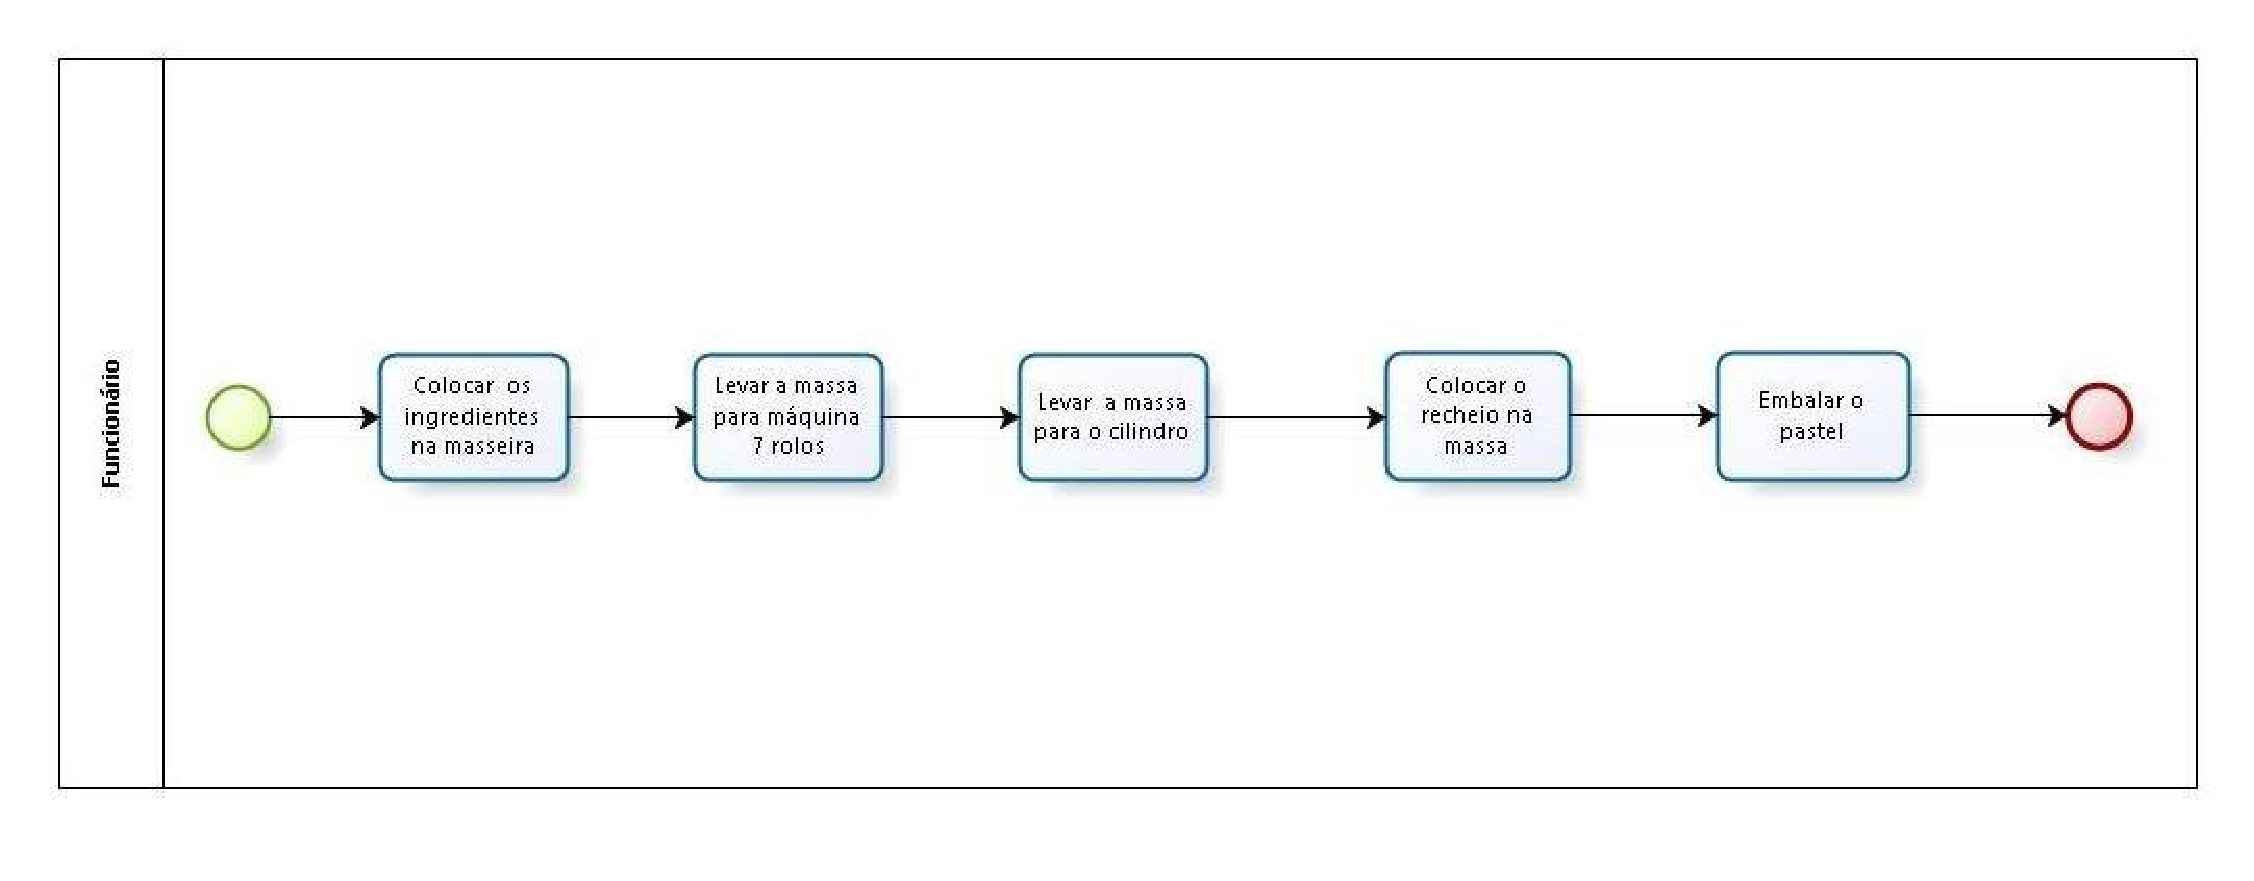
\includegraphics[width=1.1\textwidth,keepaspectratio=true,scale=0.5]{figuras/processo.eps}
    \caption{Processo.}
    \label{fig:processo}
\end{figure}

\begin{table}[H]
    \centering
      \begin{tabular}{| m{8cm} | m{8cm} |}
        \hline
        \begin{center} \textbf{Atividade} \end{center}	&	\begin{center} \textbf{Descrição} \end{center}		\\ \hline
        \textit{\textbf{Colocar os ingredientes na massieira}}	&	O funcionário introduz a matéria prima na masseira a fim de produzir a massa. \\ \hline
         \textit{\textbf{Levar a massa para máquina 7 rolos}} & A massa feita não está apta para a criação do pastel nessa etapa, sendo assim a máquina 7 rolos afina a massa, melhorando a estrutura da massa. \\ \hline
        \textit{\textbf{Levar a massa para o cilindro}} &	Para deixar a massa mais fina e consistente é utilizado a máquina de cilindro. \\ \hline
        \textit{\textbf{Colocar o recheio na masseira}}	&	Nessa etapa, a massa já está pronta para introduzir o recheio na máquina fechador automático. \\ \hline
        \textit{\textbf{Embalar o pastel}}	&	Ao final, os pasteis são embalados em pacotes, levados para camara fria e estão aptos para a venda. \\ \hline
      \end{tabular}
      \caption{Processo da Fabricação de Pastel}
      \label{tabela:processofabrica}
  \end{table}